\label{secondaries}
The secondary tracks inside the associated track sample, due to interaction of primary track with the detector material or to decays of strange hadrons, are mostly removed by the DCA cuts applied during the cut selection phase (DCA($xy$) $<$ 1 cm, DCA($z$) $<$ 1 cm).
Anyway, a small fraction of secondary tracks survives this cut, and the data correlation distributions have to be corrected for this residual contamination.
The fraction of surviving secondary tracks is evaluated via a study on the LHC17d2a$\_$fast$\_$new sample, by counting the number of tracks accepted by the selection whose corresponding generated-level track doesn't satisfy the IsPhysicalPrimary() call, and dividing this number by the total numner of accepted tracks.
The outcome of the check is reported in Figure \ref{fig:secnumber}. As it's visible, no more than 5\% secondary tracks pass the selection. Moreover, the fraction of residual secondary tracks is flat along the $\Delta\phi$ axis, as shown, for exemplary $\pt$ regions, in Figure \ref{fig:secdPhi}, where the inhomogeneities are always below 1\%.
For this reason, it is possible to directly scale the data correlation distributions by their purity fraction (i.e. 1 - secondary contamination). This is done with an associated $\pt$ dependence, due to the increase of the purity with the track $\pt$, while the purity fraction is taken flat versus the D-meson $\pt$.
The purity values that were choosen are the following:
\begin{itemize}
  \item $\pt$(assoc) $> 0.3$ GeV/c: 0.958
  \item $\pt$(assoc) $> 1$ GeV/c: 0.973
  \item $0.3 < \pt$(assoc) $< 1$ GeV/c: 0.953
  \item $1 < \pt$(assoc) $< 2$ GeV/c: 0.969
  \item $2 < \pt$(assoc) $< 3$ GeV/c: 0.982
  \item $\pt$(assoc) $> 3$ GeV/c: 0.990
\end{itemize}


\begin{figure}[h]   %da B
	\centering
	%Marianna
		  % by Fabio
	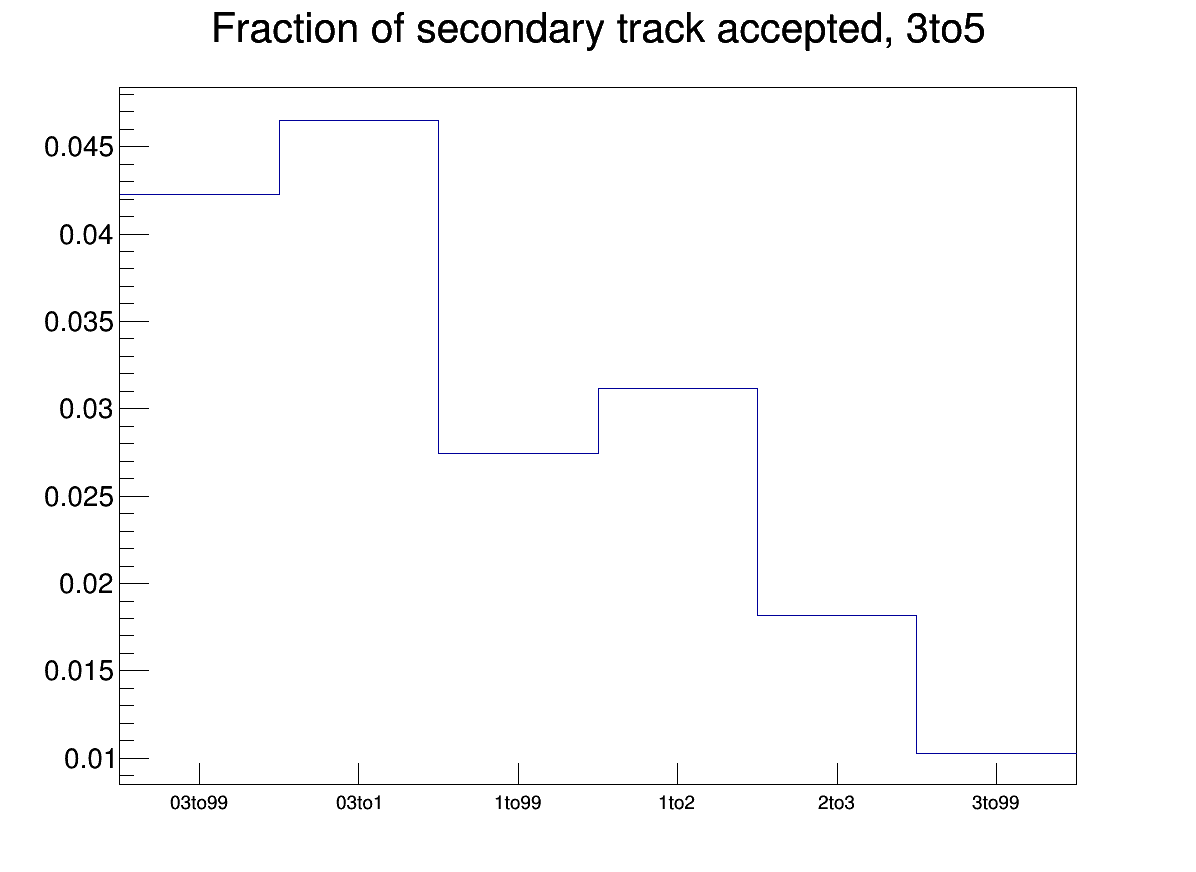
\includegraphics[width=.48\linewidth]{figures/SecTracks/FractOfSecOverTotal_3to5.png}
	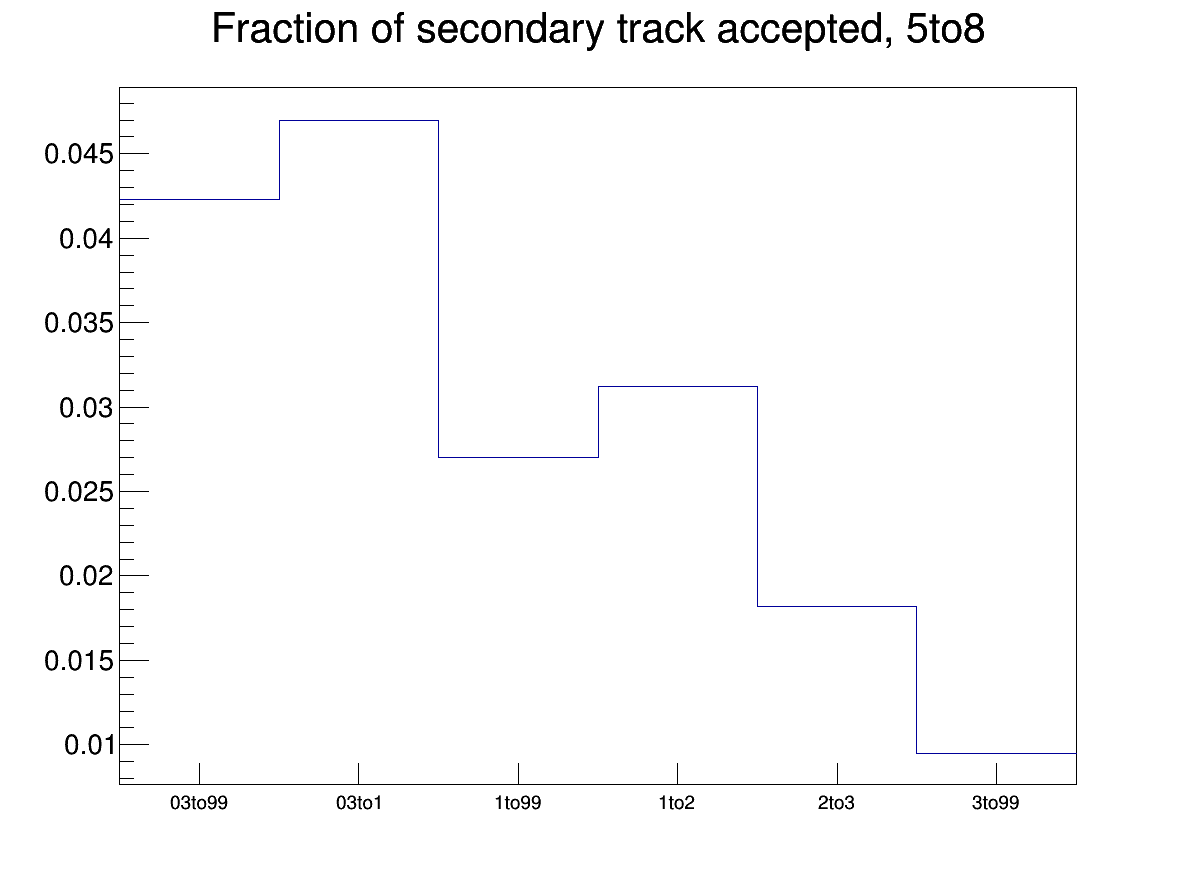
\includegraphics[width=.48\linewidth]{figures/SecTracks/FractOfSecOverTotal_5to8.png}
    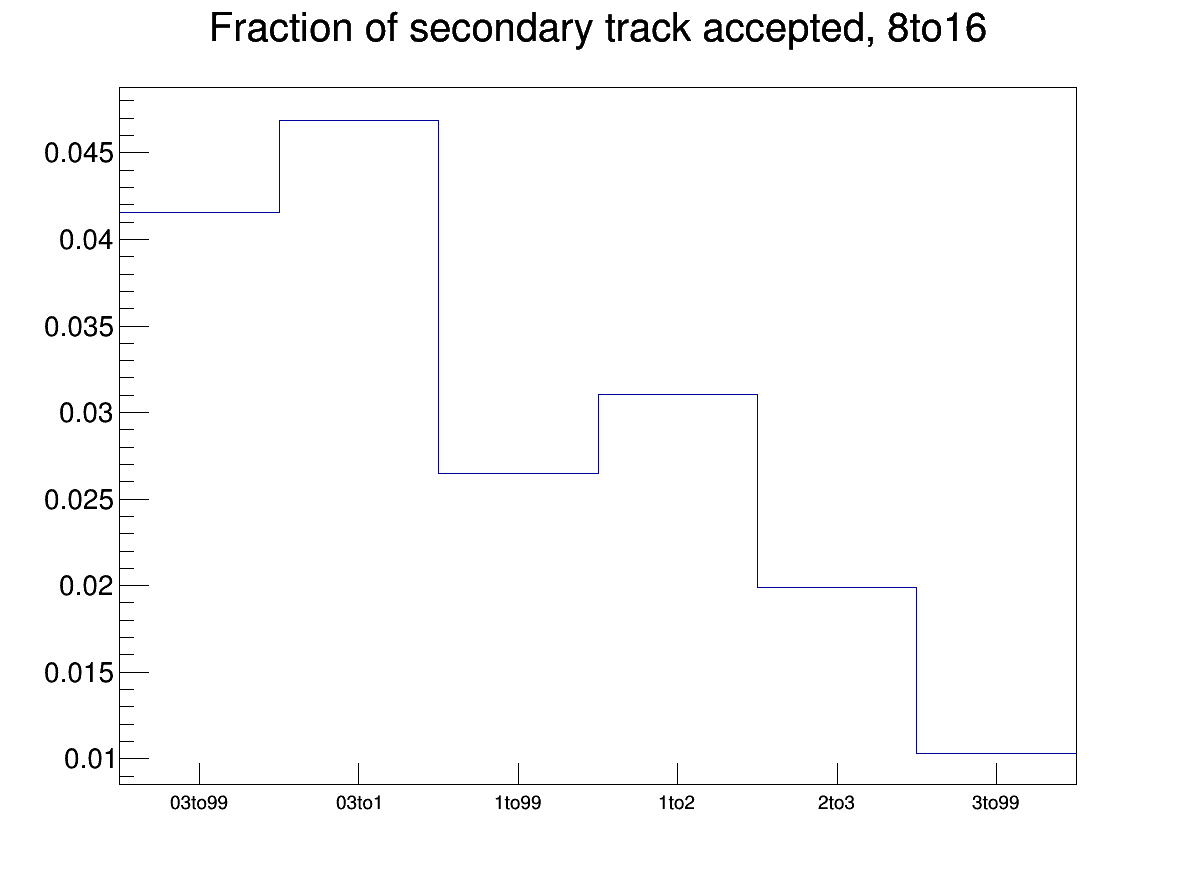
\includegraphics[width=.48\linewidth]{figures/SecTracks/FractOfSecOverTotal_8to16.png}
    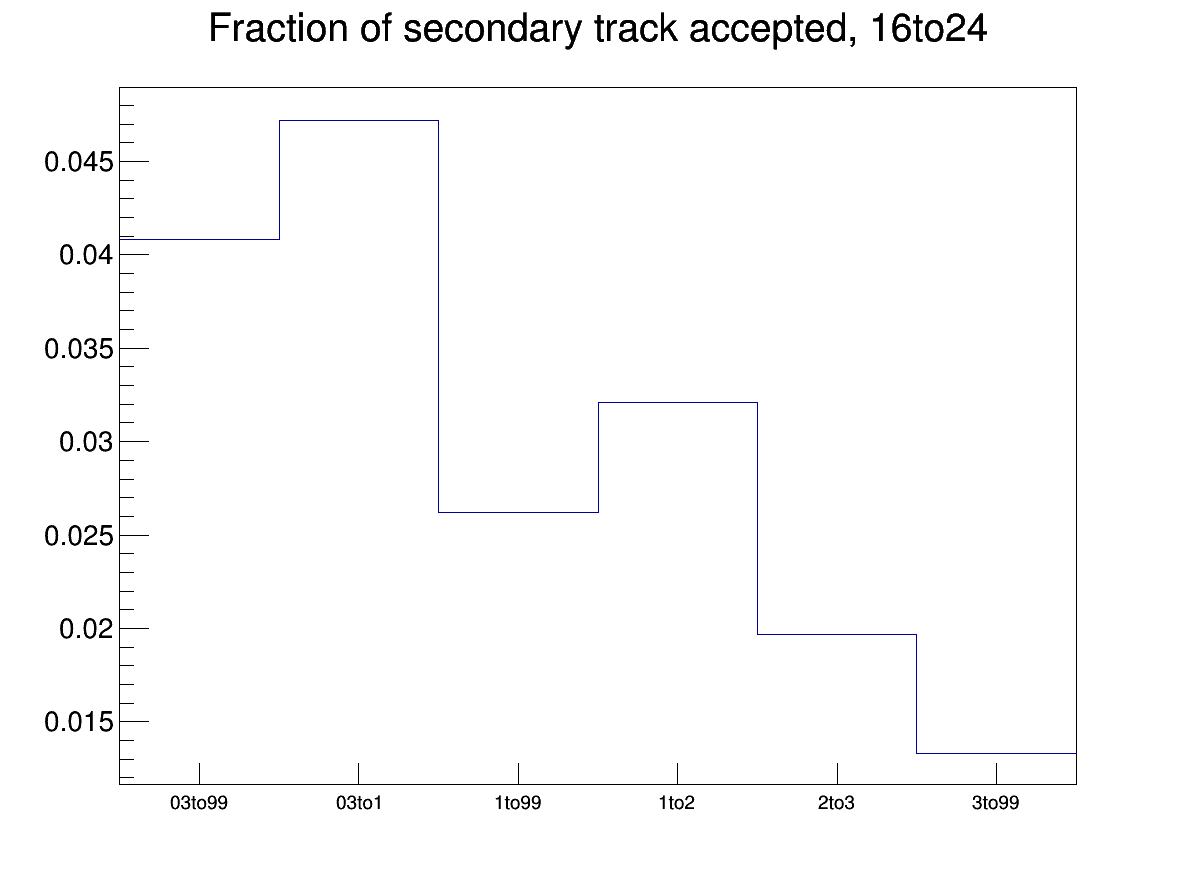
\includegraphics[width=.48\linewidth]{figures/SecTracks/FractOfSecOverTotal_16to24.png}
	\caption{Fraction of secondary tracks over total amount of tracks which pass the DCA selection. The four panel show the fractions for the D-meson $\pt$ ranges: 3-5, 5-8, 8-16, 16-24, respectively. Inside each panel, the associated track $\pt$ ranges are shown on the $x$-axis.}
	\label{fig:secnumber}	
\end{figure}

\begin{figure}[h]   %da B
	\centering
	%Marianna
		  % by Fabio
	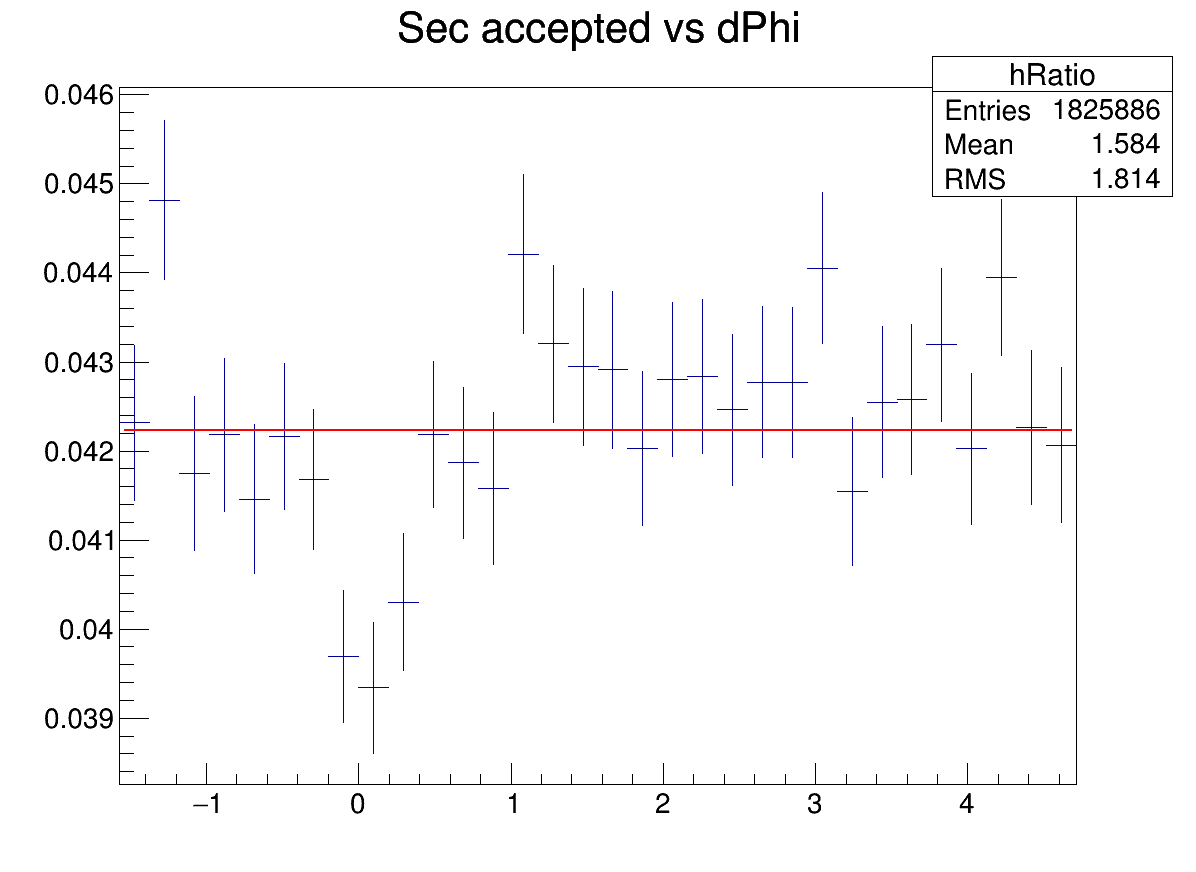
\includegraphics[width=.48\linewidth]{figures/SecTracks/DeltaPhi_3to5_03to99_RatioSecOverAll.png}
	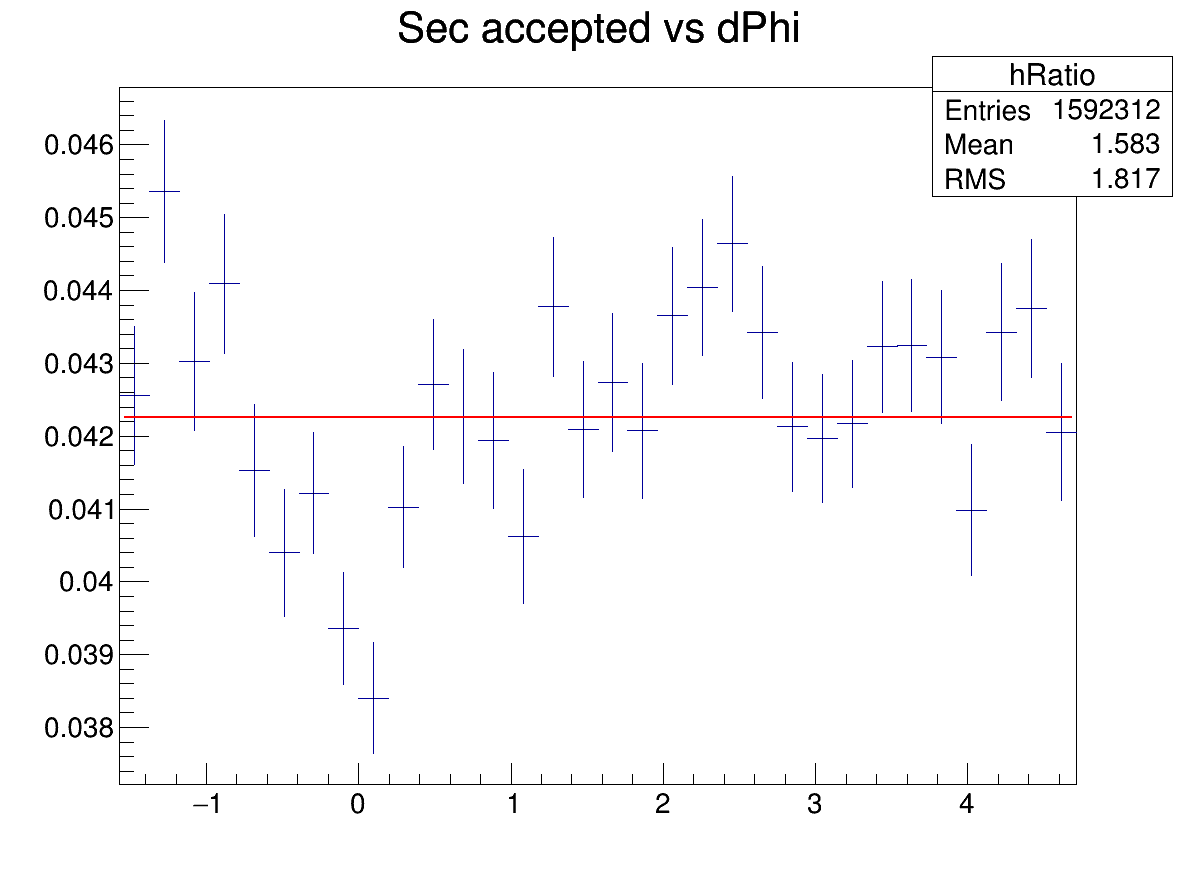
\includegraphics[width=.48\linewidth]{figures/SecTracks/DeltaPhi_5to8_03to99_RatioSecOverAll.png}
    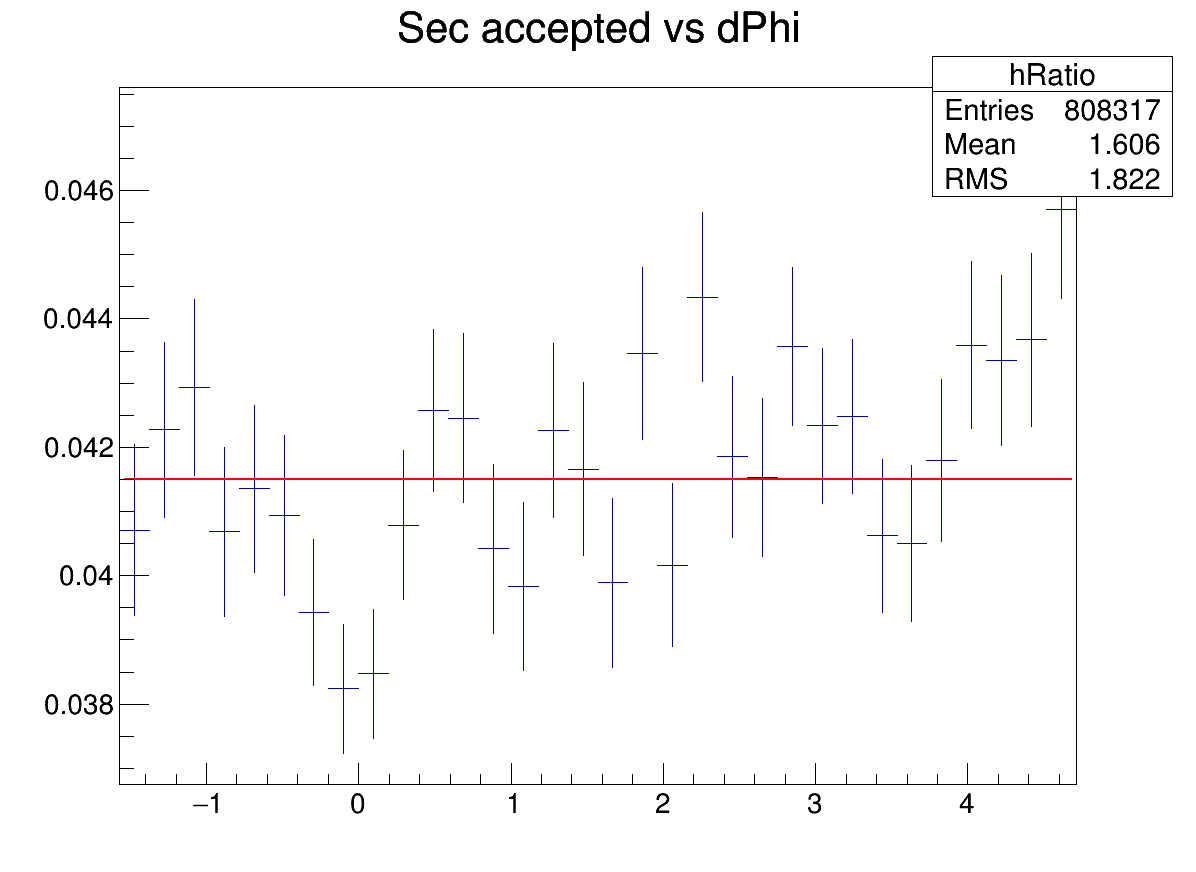
\includegraphics[width=.48\linewidth]{figures/SecTracks/DeltaPhi_8to16_03to99_RatioSecOverAll.png}
    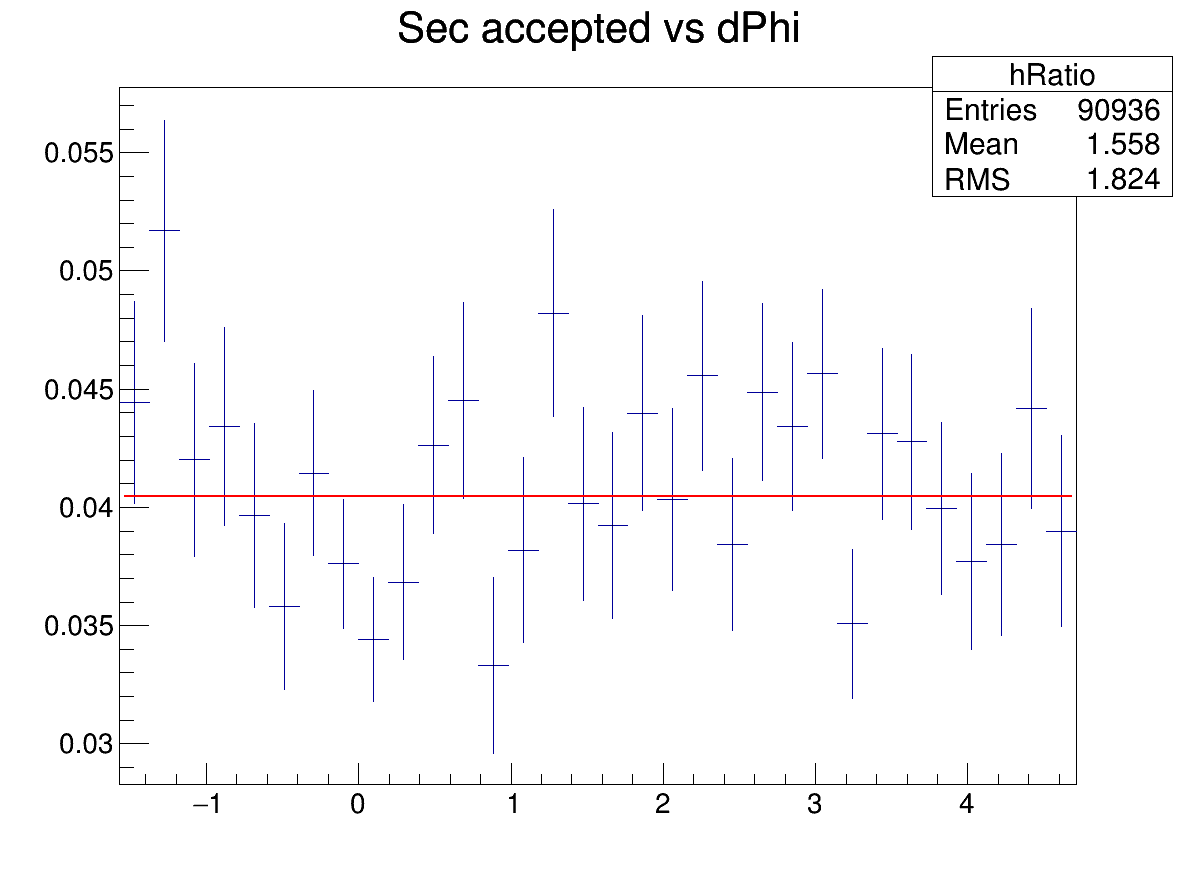
\includegraphics[width=.48\linewidth]{figures/SecTracks/DeltaPhi_16to24_03to99_RatioSecOverAll.png}
	\caption{$\Delta\phi$ dependence of the fraction of secondary tracks in the $\Dzero$-h correlation distributions. The four panel show the fractions for the D-meson $\pt$ ranges: 3-5, 5-8, 8-16, 16-24, respectively. The associated track $\pt$ ranges is the integrated one, i.e. $\pt > 0.3$ GeV/c.}
	\label{fig:secdPhi}	
\end{figure}

It was also verified with the same Monte Carlo study that applying the DCA selection rejects less than 0.2\% primary tracks (tagged as false positives) from the associated track sample, again with a flat azimuthal distribution, inducing hence a fully negligible bias on the data correlation distributions. This is shown in Figure \ref{fig:primRej}. This was also verified for specific charm-origin and beauty-origin tracks, due to their larger DCA with respect to primary tracks from light quarks. In this case, the fraction of rejected charm and beauty tracks stays below 1\% in all the kinematic ranges apart from the associated track $\pt$ regions 0.3-1 and $>0.3$ GeV/c, where the rejection can be as high as 2\%. In these kinematic ranges, though, the data correlation distributions are dominated by non-heavy-flavour tracks, as it was verified from the simulations, hence the overall bias is still contained below 1\%, thus negligible.

\begin{figure}[h]   %da B
	\centering
			  % by Fabio
	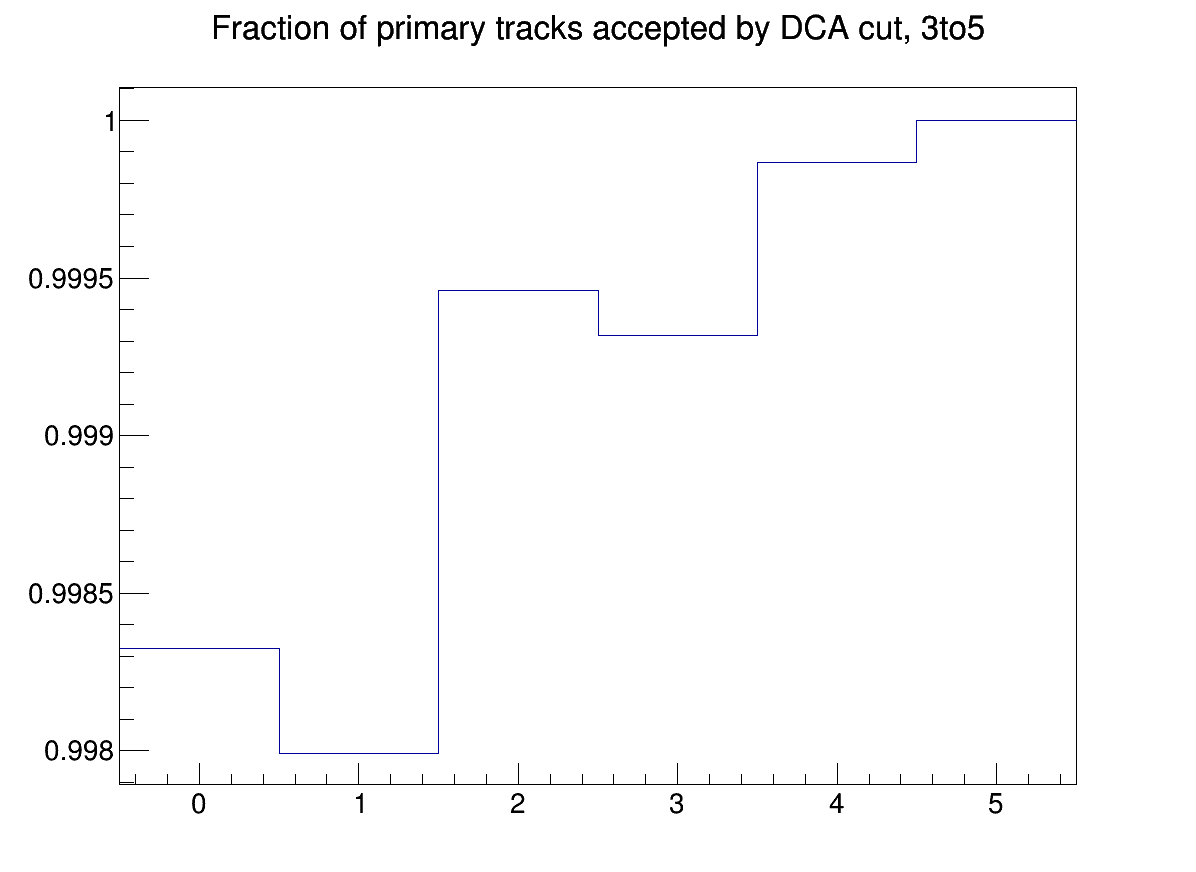
\includegraphics[width=.48\linewidth]{figures/SecTracks/FractOfPrimAccepted_3to5.png}
	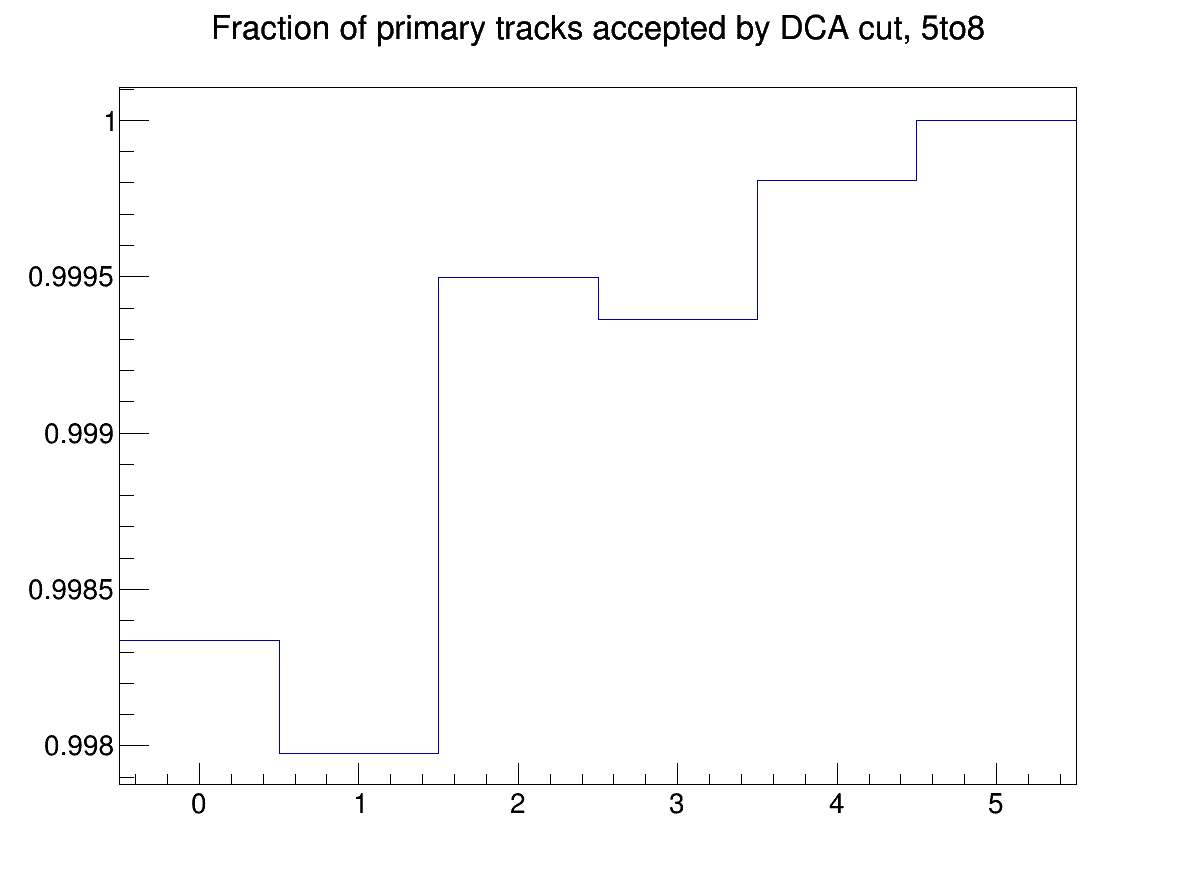
\includegraphics[width=.48\linewidth]{figures/SecTracks/FractOfPrimAccepted_5to8.png}
    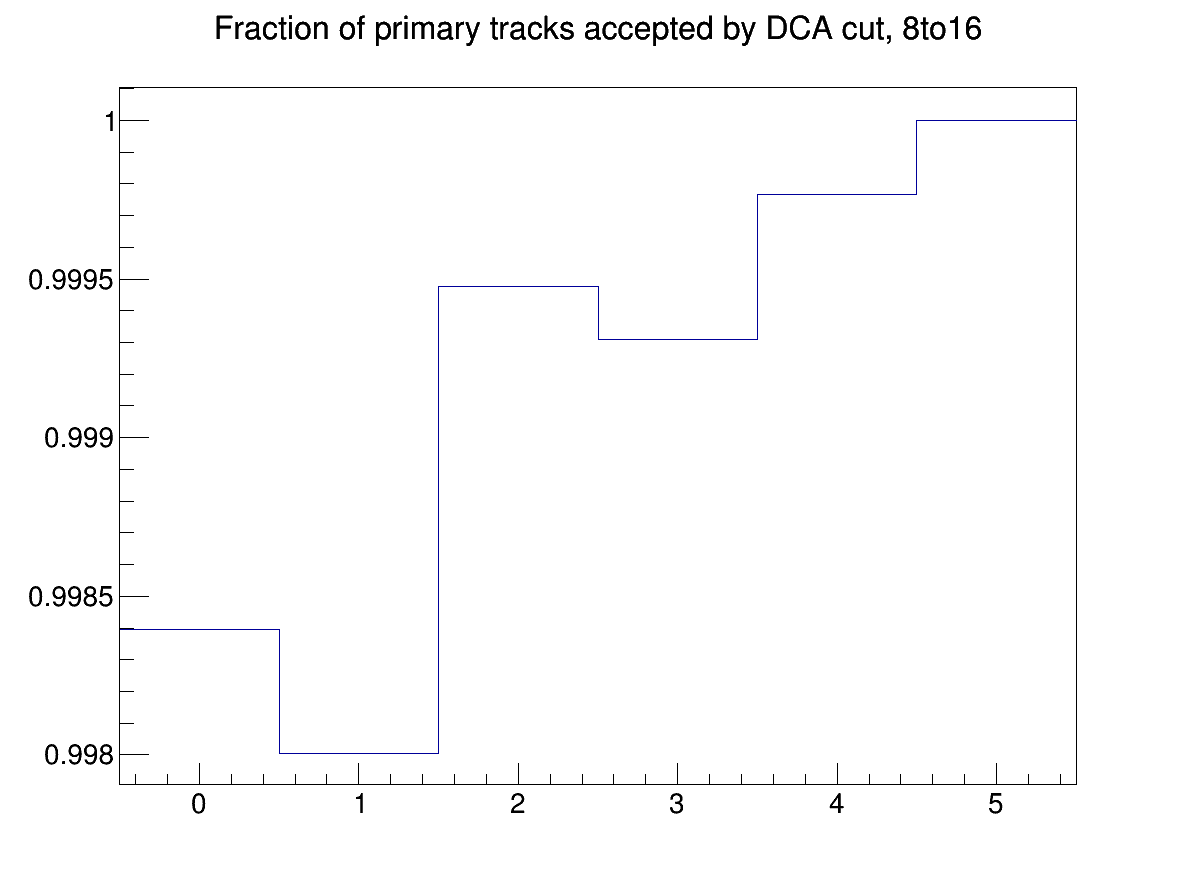
\includegraphics[width=.48\linewidth]{figures/SecTracks/FractOfPrimAccepted_8to16.png}
    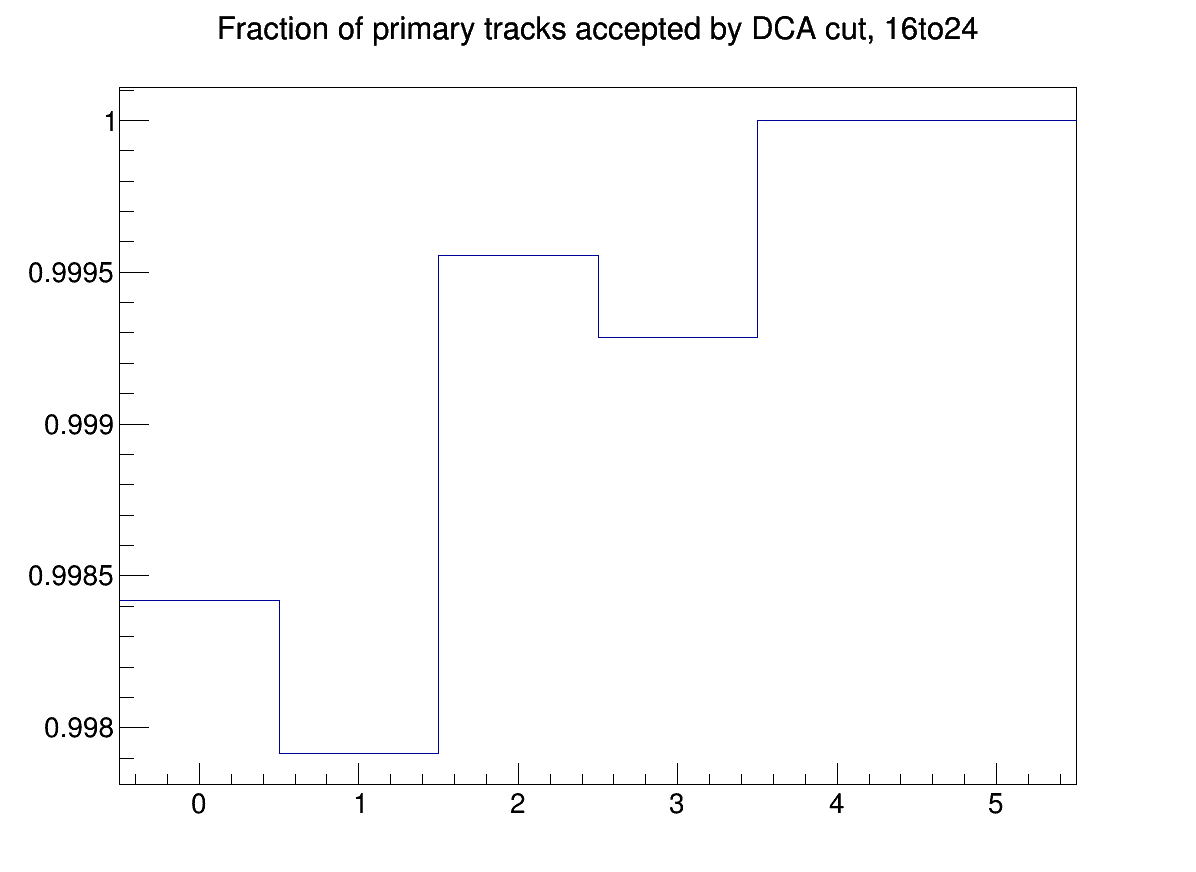
\includegraphics[width=.48\linewidth]{figures/SecTracks/FractOfPrimAccepted_16to24.png}
	\caption{Fraction of primary tracks rejected by the DCA selection. The four panel show the fractions for the D-meson $\pt$ ranges: 3-5, 5-8, 8-16, 16-24, respectively. Inside each panel, the associated track $\pt$ ranges are shown on the $x$-axis.}
		\label{fig:primRej}	
\end{figure}

These studies were performed on an enriched Monte Carlo sample, which could not fully reproduce the relative abundancies of the species. Anyway, for events with a reconstructed D-meson, this bias is expected to be minor, and only these events are used in the data analysis. In any case, the percentages obtained from the study were found to be consistent within 1\% with the outcome of the studies for the p-Pb 2013 analysis, which reassures us on the full validity of these results.

\clearpage
%\end{document}
